\chapter{Simulation}

    \section{Software choices}
        As we need to build a simulation platform, the first guess would be to use pre-existing physics engines to build our simulation such as PyBullet or Gazeboo framework that are well known in simulation field. The reason why we are building our own simulation framework is because we are not building a physics engine, but rather a mathematical solver for a specific scenario. Also by building our own implementation we can specifically add or removes modules that will analyze simpler or more complex scenarios. We also controls how valid the output is as we knows what hypothesis has been made during the implementation. With those facts, we decided to build our own framework. The choice of the programming language is determined by the tasks we need to achieve, which are characterized by mathematical solver and ease of modular design. This leaves us two main languages, Python and Matlab, both are very similar but Python is well known regarding machine learning tools available and Python would gives us more flexibility in case of future work involving machine learning analysis. Based on those points, we choose Python as a main language. 
    
    \section{Program structure}\label{sec:program_structure}
        Our framework will be built using Python 3. This allows us to create modularity in the structure of the simulation. As we can see on Figure \ref{fig:code_structure}, each physical part of the robot has its own module and implementation. Each module is responsible to respect the physical constraints of its own, to draw the module, to compute displacement given a specific input and to returns different values or points. The modules offer a great flexibility for future improvement or refinement if necessary. We have six modules that represent a simulation: \textit{bar, block, joint, robot, spring, simulation} and a main module that handle the configuration and the environment of the simulation. \\
        
        \begin{figure}
            \centering
            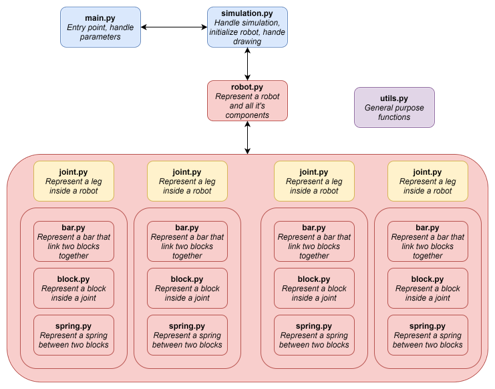
\includegraphics[width=0.8\textwidth]{images/code_structure.png}
            \caption{Caption}
            \label{fig:code_structure}
        \end{figure}
        
        \paragraph{bar}
            module represent the arms in a bistable joint. Those arms are connecting two blocks together with 4 anchors points. It is represented by two low anchors linked to the bottom block and two high anchors linked to the top block. Bar also has a length parameter. It contains functions to draw bars as output and could implement joint friction in the future if needed. 
        \paragraph{block}
            module is the basic structure of the robot, it represents one of the three blocks in the multistable joint. therefore it has a specific width, height, a center of mass location and anchors points to attach the arms. It also handles information about which block it is (bottom, middle, top) and to which actuator it is connected to, in order to have the correct representation while drawing. This module contains functions to compute position of anchors where the arms are linked in addition to the drawing functions.
        \paragraph{joint}
            module represent the multistable structure, composed of three blocks, two springs and four bars. This module allows lots of parameters, such as: joint sequence as seen in section \ref{sec:sequences}, position of the joint relatively to the main frame center of mass, initial position of the joint, arms length ($r_1, r_2$), maximum angle ($\theta_{s1}, \theta_{s2}$) and different colors. This module first initialize the position of the different sub-modules with the input constraints such as maximum angle and arms length. It also contains the different computation parts that animate the legs depending of one of the 15 implemented sequences. Those sequences are based on two simple function that take care of displacing the middle block or the top block. 
        \paragraph{robot}
            module is responsible to build the four multistable joints, the two actuators and the main frame. It contains the joints positions relative to the robot space and coordinate the actuators motions to the multistable joints. The attitude and the position of the robot is also controlled inside this module. Each time the robot is performing a displacement, the module recompute the touching points and the correct orientation of the robot. This module is also responsible of drawing the main frame and the different helps beside the robot such as the orientation of the robot.
        \paragraph{spring}
            module is used today only as a drawing part for the multistable joint. But it can handle future upgrade such as computing forces. 
        \paragraph{simulation}
            module is a top level part that is responsible to ensure the simulation is running smoothly. It receives the different parameters from the main module and create the robot from those. Once the robot initialized, simulation module can start to apply motion to the actuators and to store results of motion of the robot. It is also responsible to aggregate the different output points from the robot module to store them in a Pandas Dataframe which is saved for later use. 
        \paragraph{main}
            module is a very short module that is responsible to load the configuration file that contains the parameters of the simulation and to then load the simulation with this configuration file. 
    \section{Configuration}\label{sec:config}
        As discussed in the appendix section \ref{sec:program_structure}, the simulation is created using a configuration file. This file is use a JSON structure, which is a $key$ $value$ type. There is two main category of settings: \textit{simulation} and \textit{robot}. 
        
        The first one contains the different settings regarding the simulation process, such as \textit{actuation} field that contains the number of steps to compute, the number of cycles to simulate and the phase difference between the actuators. A phase difference of $0$° means that both actuators extend or retract at the same time. A phase difference of $180$° means that while one actuator is extending, the other is retracting itself. \textit{Draw} Boolean determine if there is drawing output produced. It can be useful to set it to false if we want to run the experiment fast and only produce data-points of positions without having a video produced each time. \textit{Camera\_robot\_ref} Boolean allows to have a fixed camera if false or to have the camera that will follow the robot motion if set to true.
        
        The second group of parameters is used to initialize robot's parameters. Each leg can be configured specifically. We have a \textit{sequence} parameter that we can set to one of the 15 sequences encoded (A-O). \todo{Setup the r1 r2 parameters}
        
    \section{Simulation process}
        The simulation process is straightforward. First we initialize the starting point of the robot and the position of each block from the four multistable legs. We also create the actuation matrix regarding the parameters and the physical constraints of the blocks. The actuators are set to run to the maximum position they can reach with the multistable joint. We also dissociate the forward motion from the backward motion, which make it easier later to know what motion to perform depending of the sequence.
        
        Once the initialization is done, we can start the simulation with a loop that will go through all the steps of the simulation. The total number of steps is equal to $cycles \cdot steps$ and for each step we will call a function to update the position of the robot and then draw the updated position. 
        
        \subsection{Update robot position}
            To update the robot position, the simulation gives first priority to moves the multistable joint individually. Each leg receive the displacement coming from the linked actuator and perform the correct motion of blocks regarding the sequence selected for each sequence. Once the motion from the legs done, we will update the attitude and the position of the robot from the position of the legs.
            We first compute the new attitude of the robot, which is represented by a pitch (y axis) and roll (y axis) rotations. To compute the angle of the robot relative to the ground, we will first sort the legs by their relative high in their own reference frame. Once done we have four possible cases, have one to four legs that are high and so that are touching the floor by default. We can resolve the case in the following way:
            \paragraph{One leg} is touching the floor. As it is not possible to get at equilibrium state on one leg, we need to look for the next leg(s) that will be touching the ground. We know that the gravity will pull the center of gravity of the robot toward the ground but it will go down with an axis of rotation that is located at the touching leg point and the rotation line will be parallel to the ground and perpendicular to the vector going from the touching leg to the center of gravity of the robot. We then look which of the remaining leg require the smallest rotation of the robot to be touching the ground plane. The smallest angle will determine which leg(s) will then also touch the floor. We now have two, three or four touching legs and we move to the specific case respectively.
            \paragraph{Two legs in diagonal} are touching the floor. So here we have either legs one and four that are touching the ground, either legs two and three. This is a specific case where the robot is at an equilibrium state and so we can compute the roll and pitch inclination. 
            \paragraph{Two legs not in diagonal} are touching the floor, in this case, we need to find a third or fourth point off contact. The process is similar than in the one leg case. We have the center of gravity of the robot that will go down and rotate around an axis. This axis is represented by a line going from the two legs that are already touching the floor. We then find the leg that require the smallest angle to touch the ground. We then move to the three legs case or the four legs case if both other legs are touching the floor. 
            \paragraph{Three legs} are touching the floor. To compute the pitch and roll angle, we first define the plane with three legs and compute the angle difference with the flat plane. 
            \paragraph{Four legs} are touching the floor. It is very similar than the three leg process, we just select three legs that will create our plane to compute the roll and pitch.
            \\
            
            We know how many legs are now touching the ground and how the robot is level relatively to the ground. Those information are important to compute the weight distribution on each touching leg and then to compute which leg is \textit{anchored} to the ground. To determine the weight distribution we need to satisfy two constraints. First is that the sum of the reaction forces need to equal the weight of the robot. Second, we need to have the sum of the momentum to be equal to zero too. Once we know the reactions forces we will that the assumption that the highest reaction force will anchor the leg. The others legs will move freely on the surface. 
            
            
            